\title{Benchmarking a Sentiment Analysis Algorithm Using Hadoop on Multiple 
Platforms}


\author{Min Chen}
\affiliation{%
  \institution{Indiana University}
  \streetaddress{School of Informatics, Computing, and Engineering}
  \city{Bloomington}
  \state{IN}
  \postcode{47408}
}
\email{mc43@iu.edu}

\author{Gregor von Laszewski}
\affiliation{%
  \institution{Indiana University}
  \streetaddress{Smith Research Center}
  \city{Bloomington}
  \state{IN}
  \postcode{47408}
}
\email{laszewski@gmail.com}

\author{Bertolt Sobolik}
\affiliation{%
  \institution{Indiana University}
  \streetaddress{School of Informatics, Computing, and Engineering}
  \city{Bloomington}
  \state{IN}
  \postcode{47408}
}
\email{bsobolik@iu.edu}


% The default list of authors is too long for headers}
\renewcommand{\shortauthors}{M. Chen, G. v. Laszewski, B. Sobolik}


\begin{abstract}
A sentiment analysis algorithm is run on several Hadoop
configurations: in pseudo-cluster mode on an Ubuntu 16.04 virtual
machine on a MacBook Pro with and without YARN, in pseudo-cluster mode
in a Docker container on various personal computers and on
Futuresystems Echo, in a cluster created using Docker Compose on
various personal computers and on Futuresystems Echo, and in a cluster
created using Docker Swarm on various Futuresystems Echo. Performance
tests are natural language processing based sentiment analysis on
movie reviews (Polarity 2.0) implemented under MapReduce framework
using Hadoop Streaming. Configurations are described in detail and
steps to recreate them are outlined. In an appendix, steps toward
creating a Hadoop cluster on five networked Raspberry Pi 3 model B
computers in a repeatable and scalable fashion, automating as much of
the setup process as possible are detailed and next steps are
discussed.
\end{abstract}

\keywords{hid-sp18-419, hid-sp18-405, Hadoop, Docker, Futuresystems}


\maketitle

\section{Introduction}\label{s:intro}
\TODO{Write an introduction.}


\section{Technology Used}\label{s:techused}

This section describes the technologies that has been utilized
throughout the project. These technologies can be grouped into several
groups: Hadoop, Docker, personal computers, and cloud platforms.

\subsection{Hadoop}
Apache Hadoop is a software library that allows for processinglarge data sets 
in a distributed computing environment~\cite{hid-sp18-405-hadoop-wiki}. 
Inspired by the Google File 
System~\cite{hid-sp18-405-ghem2003goolefilesystem} and MapReduce 
programing model~\cite{hid-sp18-405-dean2008mapreduce} developed at 
Google, Hadoop was initially released in December 2011. ``Rather than rely 
on hardware to deliver high-availability, the library itself is designed 
to detect and handle failures at the application layer, so delivering a 
highly-available service on top of a cluster of computers, each of which may 
be prone to failures''~\cite{hid-sp18-405-hadoop-official}.

The core of Hadoop include the following components: Hadoop Common, 
Hadoop Distributed File System (HDFS), Hadoop YARN and Hadoop 
MapReduce~\cite{hid-sp18-405-hadoop-official}. There is also a large variety 
of Hadoop-related projects at Apache covering aspects such as machine 
learning (Mahout), data warehousing (Hive), data serialization (Avro), and 
databases (Hbase, Cassandra) etc. Alla these components are available
via the Apache open source license. The high level basic Hadoop architecture 
in a distributed cluster with one Master Node and two Worker Node is 
illustrated in Figure~\ref{f:hadoop-high}.

\begin{figure*}[!ht]
	\centering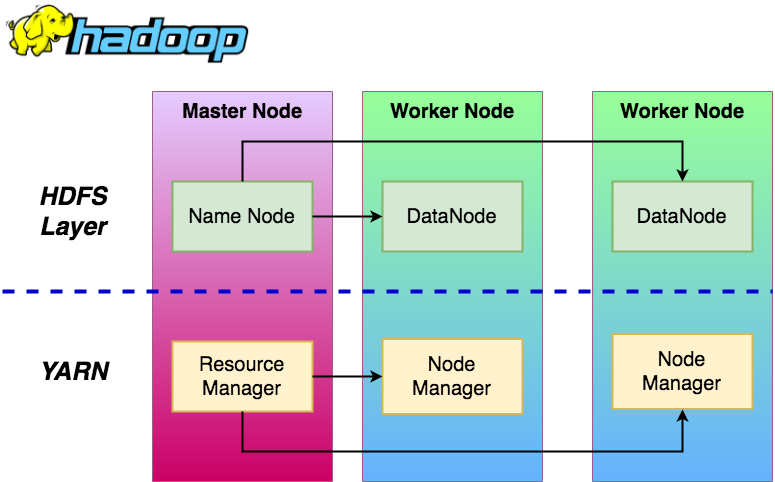
\includegraphics[width=\columnwidth]{images/hadoop.png}
	 \caption{Hadoop High Level Architecture}\label{f:hadoop-high}
\end{figure*}

\paragraph{HDFS} Hadoop Distributed File System stores metadata and 
application data separately: metadata are stored on the NameNode (usually 
sitting on the Master Node) and application data are distributively stored on 
Datanodes and the communication between them are through TCP-based
protocols~\cite{hid-sp18-405-shvachko2010hdfs}. Instead of storing one 
copy, data is replicated on multiple DataNodes to ensure high-availability. 

\paragraph{MapReduce} Hadoop MapReduce is an ``implementation of the 
MapReduce programming model for large-scale data 
processin''~\cite{hid-sp18-405-hadoop-official}. ``Users specify a map 
function that processes a key/value pair to generate a set of intermediate 
key/value pairs, and a reduce function that merges all intermediate
values associated with the same intermediate 
key''~\cite{hid-sp18-405-dean2008mapreduce}. As illustrated in 
Figure~\ref{f:hadoop-high}, Master Node will have a JobTracker who 
distributes MapReduce tasks to nodes in the cluster. On the other hand, 
TaskTracker within each node is monitored by the Jobtracker. In case of a 
failure reported by a TaskTracker, the Jobtracker may reschedule the work to 
some other nodes~\cite{hid-sp18-405-hadoop-jobtracker}. 

\paragraph{YARN} Hadoop YARN provides resource management for the 
Hadoop cluaster~\cite{hid-sp18-405-hadoop-official}. As shown in 
Figure~\ref{f:hadoop-high}, based on application demand, priorities,
and resource availability, the Resource Manager dynamically allocates
containers (logical bundle of resources different from Docker containers) to 
applications to run on particular nodes~\cite{hid-sp18-405-vavi2013yarn}. It 
interacts with Node Manager on each nodes, whose job is to monitor 
resource availability, report faults, and manage container 
lifecycles~\cite{hid-sp18-405-vavi2013yarn}. 

\paragraph{Hadoop-streaming} Although Hadoop is written in Java as well 
as most of its applications, Hadoop streaming, a tool that comes with the 
Hadoop distribution, ``allows creating and running MapReduce jobs with any 
executable or script as the mapper and/or the 
reducer''~\cite{hid-sp18-405-hadoop-streaming}. In this project, all the 
mappers and reducers are written in Python and passed to 
Hadoop-Streaming. One drawback for this approach is that if the executable 
contains outside packages, they need to be zipped in a flat way and passed 
to each job containers for a special import before use. 
It will be discussed in Section\label{s:algorithm} that some of the linguistic 
features in this project are omitted due to the difficulties of transporting and 
loading necessary packages and corpus. 


\subsection{Docker}
Docker is a technology performs operating-system-level virtualization, that 
allows applications to run in containers instead of full 
VMs~\cite{hid-sp18-405-docker-wiki}~\cite{las18handbook}. It leverages 
control groups and name space
isolation in the Linux kernel. Containers start up much faster than
VMs and are supported by all the major public cloud
vendors~\cite{Foster:2017:CCS:3158276}. The most current stable
release of Docker Community Edition is used for this project
(18.03.0-ce).

\paragraph{Docker Compose} Compose is a tool coming with Docker that 
helps define and manage applications or clusters with multiple Docker 
containers~\cite{hid-sp18-405-docker-compose-doc}. Docker Compose 
provides multiple isolated environments on a single host, which is utilized in 
this project that Hadoop cluster could be deployed on a single virtual and/or 
physical machine with Master Node and Worker Nodes running on separate 
containers. Further, the scalability feature of Docker Compose allows the size 
of the cluster to be adjusted at run time without stopping the cluster. When 
service is restarted, and configuration files are not changed for some 
containers, Compose re-uses these existing containers thus increasing the 
speed of adjustment in a dynamic 
environment~\cite{hid-sp18-405-docker-compose-doc}.

\paragraph{Docker Swarm} A group of physical or virtual machines running 
Docker Engine can be joined into a cluster called Docker Swarm. Each 
machine is referred to as node. One node in the cluster will be the head or 
manager of the swarm which is the only node communicating with outside 
client and received execution instructions. It will then coordinate and pass 
instructions to other worker nodes. In the cloud platform, FutureSystem 
Echo we are using for this project, five physical server are in Docker Swarm 
mode with one head and four workers. Key features of Docker Swarm 
includes cluster management integrated with Docker Engine, decentralized 
design, scaling, load balancing and rolling 
updates~\cite{hid-sp18-405-docker-swarm-doc}. Stack of services could be 
deployed on a Swarm cluster using the same YAML file as in Docker 
Compose. User could pass a single command to start, scale or stop the 
services to the head node, who will coordinate among the Swarm cluster with 
optimized load balancing. 

\subsection{VirtualBox}
VirtualBox is software from Oracle that allows one to run x86 and
AMD64/Intel64 VMs on personal computers. It is used in this project
for running VMs in Hadoop setups and for burning custom images for the
Raspberry Pis discussed in Section~\ref{s:appendix}. Add-ons include
Guest Additions, which allow one to cut and paste between the VM and
the host, and the VirtualBox Extension Pack that allows mounting
peripherals on USB 3.0~\cite{hid-sp18-419-virtualbox}.

\subsection{Personal Computers}\label{ss:pcs}
\paragraph{Macbook Pro (15-inch, 2017)}
\begin{itemize}
\item Operating system: macOS Sierra 10.12.6 
\item Processor: 3.1 GHz Intel Core i7
\item Memory: 16 GB 2133 MHz LPDDR3
\item Graphics: Intel HD Graphics 630 1536 MB
\item Periphals
\begin{itemize}
\item HyperDrive - USB Type-C Hub (has microSD card slot)
\item Insignia - USB Type-C to Gigabit Ethernet Adapter (to connect to switch)
\end{itemize}
\item Software
\begin{itemize}
\item VirtualBox 5.2.8 with Guest Additions and the VirtualBox Extension Pack for USB 3.0 support.
\end{itemize}
\end{itemize}

\paragraph{Macbook Pro (13-inch, 2015)}
\begin{itemize}
	\item Operating system: macOS High Sierra 10.13.4 
	\item Processor: 2.7 GHz Intel Core i5
	\item Memory: 8 GB 1867 MHz DDR3
	\item Graphics: Intel HD Graphics 6100 1536 MB
\end{itemize}

\paragraph{Acer Laptop (Aspire 4830)}
\begin{itemize}
	\item Operating system: CentOS Linux 7 (Core)
	\item Processor: Intel (R) Core (TM) i5-2430M CPU @2.40GHz
	\item Memory: 16 GB 1600 MHz DDR3
\end{itemize}

\paragraph{Asus Desktop}
\begin{itemize}
	\item Operating system: Windows 7 Professional
	\item Processor: Intel (R) Core (TM) i5-4690K CPU @3.50GHz
	\item Memory: 16 GB 1600 MHz DDR3
	\item Software
	\begin{itemize}
		\item VirtualBox 5.2.8
	\end{itemize}
\end{itemize}

\subsection{Cloud Platforms}
\paragraph{FutureSystem Echo}


\section{Data}\label{s:data}

The data used for the project is the Polarity Data 2.0, which is a
dataset of movie reviews, first used by Bo Pang and Lillian
Lee~\cite{hid-sp18-405-sentiment-pang2004asentimental}~\cite{hid-sp18-405-sentiment-pang2002thumbs}.
The dataset includes 1000 positive and 1000 negative processed
reviews, which are labelled with respect to their overall sentiment
polarity.

Each of the review is in a format of text file, and each of the single
line in a file is corresponding to a sentence. Further, every token
(which includes single word, punctuation marks, numbers) has been
separated by space. For example, Figure~\ref{f:data} shows several
lines in one of the movie reviews with line number on the right, which
illustrate the two features mentioned above. These features play an
important role in the sentiment analysis algorithm especially under
map-reduce framework, which will be discussed in details in
Section~\ref{s:algorithm}.
\begin{figure*}[!ht]
	\centering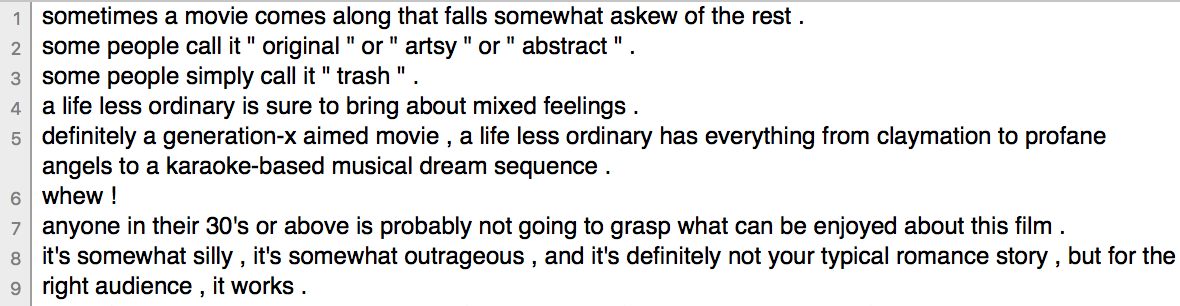
\includegraphics[width=\columnwidth]{images/polarity-data.png}
	\caption{Example Data File}\label{f:data}
\end{figure*}

The data is directly pulled from the
source~\cite{hid-sp18-405-sentiment-data} and then split into training
and testing sets according to a ratio of 8:2. The authors also keep
the original ratio of positive and negative reviews in both the
training and testing data sets. As a result, there are 1600 reviews
(800 positive and 800 negative) in the training data set and 400
reviews (200 positive and 200 negative) in the testing data set. The
splitting process is done by using the random sort functionality in
bash with a fixed random seed to ensure consistency of performance
benchmarking on different platforms.


\section{Algorithm}\label{s:algorithm}

This section introduces the algorithm used to classify the overall
sentiment of the movie reviews in the benchmarking process. The
algorithm is a modified version from Pang and
Lee~\cite{hid-sp18-405-sentiment-pang2004asentimental} and also
explained in details by Jurafsky and
Martin~\cite{hid-sp18-405-sentiment-jurafsky2009}.

\subsection{Baseline algorithm}\label{ss:base}

The baseline algorithm contains the following steps:

\begin{enumerate}
	\item Tokenization
	\item Feature Extraction
	\item Classification
\end{enumerate}

\paragraph{Tokenization}
As mentioned in Section~\ref{s:data}, every token (which includes
single word, punctuation marks, numbers) has been separated by space
in the text files. Therefore, we just need to split the text strings
with space to perform tokenization rather than use sophisticated
tokenizers. This saves space and running time as well as the
complication of loading python packages for hadoop worker nodes in
hadoop-streaming. However, in more general settings with text data,
non-trivial tokenization step needs to be performed before other type
of text processing.

\paragraph{Feature Extraction}
The main feature that we use is the words contained in the documents,
however, there are several options mentioned by Jurafsky and
Martin~\cite{hid-sp18-405-sentiment-jurafsky2009}:
\begin{enumerate}
	\item All tokens
	\item Removing stoplist words
	\item Removing punctuation tokens
	\item Using only adjectives
	\item Unify tokens with lemmas
	\item Negation treatment
\end{enumerate}
In this project, we applied stoplist words removal, punctuation tokens 
removal and negation treatment. 

Stoplist is the list of words that are considered to be commonly used
across documents regardless of sentiments thus adding little value in
classification tasks. We removed stoplist words according to the
english stopwords module from the python package: NLTK
corpus~\cite{hid-sp18-405-sentiment-stopworddoc}. Punctuation removal
is done by using python string
module~\cite{hid-sp18-405-sentiment-punctuationdoc} supplemented by
self-defined regular expression. We applied a basic negation treatment
by adding a NOT\_ prefix to every token that follows a negation word
and not separated by any punctuation tokens. For example: I really do
not like the movie becomes: I really do not Not\_like Not\_the
Not\_movie. This method is used by Das and
Chen~\cite{hid-sp18-405-sentiment-das2001yahoo} as well as Pang, Lee,
and Vaithyanathan~\cite{hid-sp18-405-sentiment-pang2002thumbs}.

We did not apply the option of using adjectives only due to the result
provided by Pang and his
colleges~\cite{hid-sp18-405-sentiment-pang2004asentimental} that
adjectives only does not provide a better results than including all
words. In fact, the accuracy dropped by on average 2\% in the testing
phase when we implemented the algorithm. We also did not apply
lemmatization for all the tokens. Although lemmatization would
increase the accuracy by around 2\% in one of the authors previous
studies, it requires ontologies such as wordnet and including the
wordnet corpus with lemmatizer is adding much complication to the
hadoop-streaming. We tried to follow the instructions
online~\cite{hid-sp18-405-hadoopstreaming-nltk}~\cite{hid-sp18-405-hadoopstreaming-corpus}
to pass python package (NLTk) and corpus (wordnet) as zipped files
from name nodes to data nodes in mapreduce tasks but the package can
be passed but not loaded and corpus cannot be passed. This issue could
be studied and solved in future projects.

Pang, Lee, and
Vaithyanathan~\cite{hid-sp18-405-sentiment-pang2002thumbs}, also
considered different set of features such as bigrams, combination
(back up) of bigrams and unigrams, top-unigrams etc. For simplicity,
we chose to only use unigram models i\.e\. single tokens.

\paragraph{Classifier}
We  used Naive Bayes as the classifier. The formulation is given as:
\begin{equation}\label{eq:nb}
c_{NB}=\text{argmax}_{c_j \in C} P(c_j) \prod_{i \in positions} P(w_i|c_j)
\end{equation}

where in this case, $j \in \{positive, negative\}$, also for this
movie review dataset, we know the prior probabilities:
$P(c_{positive})=P(c_{negative})=0.5$

\paragraph{Smoothing}
To avoid the problem that the probability of some token in the 
training/testing document is zero. We use the add-one smoothing or Laplace 
smoothing in this case:
\begin{equation}\label{eq:sm}
P(w|c) = \frac{count(w,c) + 1}{count(c) + |V|}
\end{equation}

Figure~\ref{f:algo} is the algorithm we implemented summarized by Jurafsky 
and Martin:
\begin{figure}[!ht]
		\centering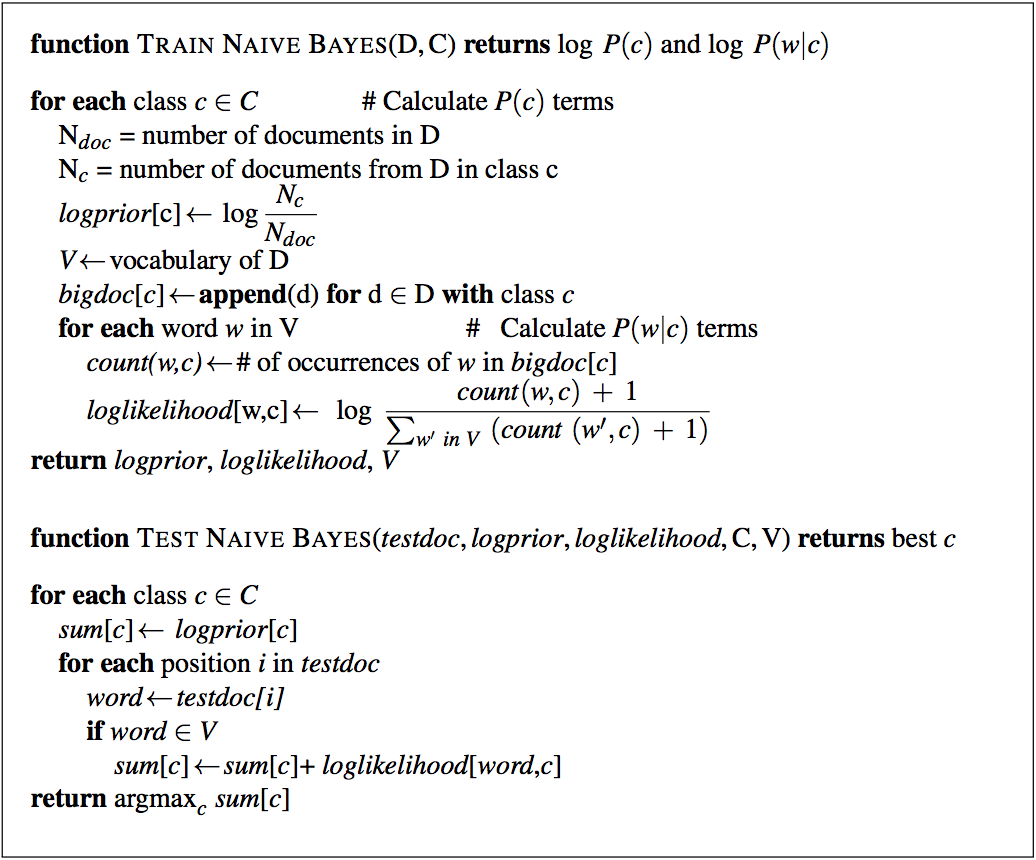
\includegraphics[width=\columnwidth]{images/algorithm.png}
		\caption{Naive Bayes for Sentiment 
		Analysis~\cite{hid-sp18-405-sentiment-jurafsky2009}}\label{f:algo}
\end{figure}

\subsection{Implementation Using MapReduce}

As illustrated in Equation~\ref{eq:nb}, Equation~\ref{eq:sm}, and
Figure\ref{f:algo}, the Naive Bayes classification algorithm is based
on comparing posterior probability. The likelihood of each single
valid token can be calculated by aggregating the count of this token
among the training documents for the two classes positive and
negative. The the likelihood of a testing document is an aggregation
of the likelihood of each valid token within that document. Therefore,
both training and testing process can be implemented in a MapReduce
framework to facilitate the process of counting tokens and
aggregation. The implementation is summarized in Figure~\ref{f:mapreduce}

\begin{figure}[!ht]
	\centering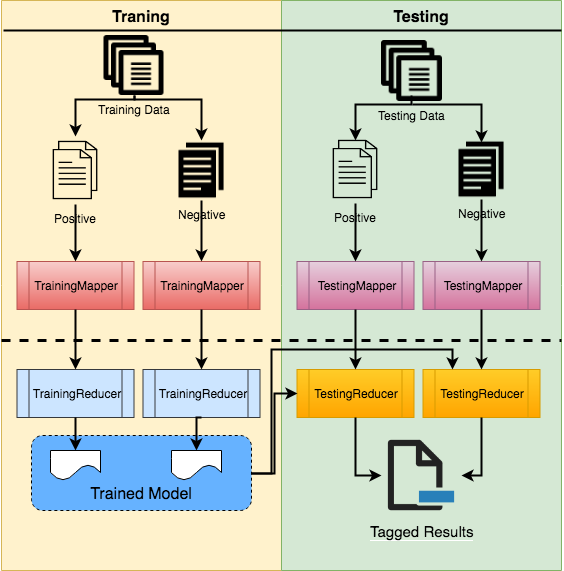
\includegraphics[width=\columnwidth]{images/mapreduce.png}
	\caption{MapReduce Implemenation of the Algorithm}\label{f:mapreduce}
\end{figure}

There are two MapReduce jobs in the training process, one for training
on positive-labelled documents and the other for negative-labelled
documents.  $count(w,c)$ in Equation~\ref{eq:sm} shows the necessity
to count the tokens according to the classes, which are positive and
negative in this task.  During the training on positive-labelled
documents, the TrainingMapper python code will read in each positive
movie reviews in the training set through standard input, filter valid
tokens (removing stoplist words, punctuation, adding negation, see
Subsection\ref{ss:base}) and print to the standard
output. The read-in process is done on a line-by-line basis using a Python 
generator. This is achievable because the data is formatted in the way that 
each line is one sentence (see Section~\ref{s:data}), thus no sentence 
splitting is accomplished by line breaks. TrainingReducer python code will 
take these standard output
performing aggregation by tokens. The result is a dictionary-like text
file containing number of occurrence for each valid token in the
positive training set. The negative training documents will be
processed in a similar way.

In the testing process, each testing document is analyzed
separately. The TestingMapper will read in the one document, perform
the same filter to keep valid tokens and print to standard output. The
testingReducer will read in both this standard output and the two
results files from the training process, calculating the likelihood of
each valid token in this document according to the smoothing formula
given by Equation~\ref{eq:sm} before getting posterior probability
through aggregation according to Equation~\ref{eq:nb}. Then for each
document, there will be two posterior probabilities, positive and
negative. The document will be assigned to the one with higher
probability. The final output will be a text file and each line is the
testing document name with its classification label. In the actual
implementation, we performed the testing process using two MapReduce
jobs, one for the testing data that are actually positive, the other
for the testing data that are actually negative. This is essentially
the same as performing testing process on each document blindly and
then verify the results. However, it is easier to calculate the
accuracy of the algorithm.
 
In summary, we used python codes to implement two mappers
(TrainingMapper and TestingMapper) and two reducers (TrainingReducer
and Testingreducer) to perform 4 MapReduce jobs for the training and
testing processes. For the fixed random seed mentioned in
Section\ref{s:data}, we achieved the following results: out of the 200
positive testing data, 162 are correctly labelled; out of the 200
negative testing data, 168 are correctly labelled. Therefore, the
overall accuracy of the algorithm is 82.5\%. This is acceptable
compared to the result achieved by Pang, Lee, and Vaithyanatha, which
is illustrated in Figure\ref{f:pang-result}.
% 
%\begin{figure}[!ht]
%	\centering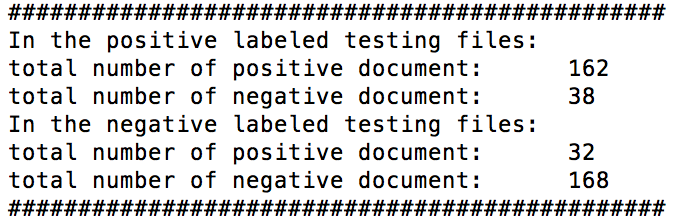
\includegraphics[width=\columnwidth]{images/algoresult.png}
%	\caption{Results of the Algorithm}
%	\label{f:algoresult}
%\end{figure}

\begin{figure}[!ht]
	\centering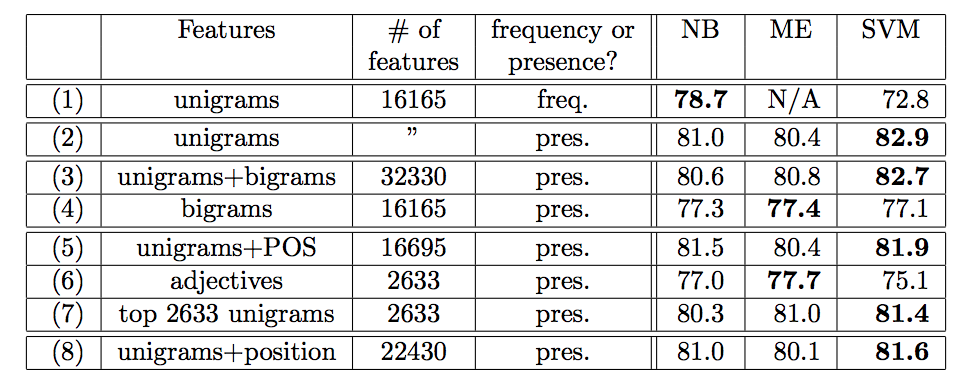
\includegraphics[width=\columnwidth]{images/pang-result.png}
        \caption{Results
	from Pang, Lee, and Vaithyanatha
	(2002)~\cite{hid-sp18-405-sentiment-pang2002thumbs}}\label{f:pang-result}
\end{figure}


\section{Hadoop Deployment}\label{s:hadoopdep}

For the entire project, we chose the current stable release of Hadoop, version 
2.9.0. For the convenience of benchmarking across platforms, we adopted a 
fixed set of configuration files for all of our installations. For example, the 
value of dfs\.replication is set to 3, which means that 3 copies of the data will 
be stored in the HDFS. In addition, physical memory limit for each map task 
and reduce task is set to 1024MB, with the ratio of virtual memory to physical 
memory allowed set to 2.1. Therefore, the virtual memory limit for each map 
task and reduce task is 2150MB. 

Hadoop can be configured to run in three modes: Standalone Mode, 
Pseudo-Distributed Mode and Fully-Distributed 
Mode~\cite{hid-sp18-405-hadoop-singlenode}. 
\begin{itemize}
	\item Standalone Mode: In this Mode, Local file system instead of HDFS is 
	used. Resource Manager, Node Manager and all other processes are 
	running not only in one virtual machine but in one single Java Virtual 
	Machine (JVM).
	\item Pseudo-Distributed Mode: HDFS is used, NameNode, DataNode, 
	ResourceManager and NodeManager are in the same virtual machine but in 
	different JVMs. 
	\item Fully-Distributed Mode: This is the mode that Hadoop clusters can be 
	ranging from a few nodes to large clusters with thousands of nodes. Each 
	node (worker) will be on different virtual/physical machines and they all 
	have DataNode and NodeManager running as seperate JVMs.
\end{itemize}
In this project, we deployed Hadoop in Pseudo-Distributed Mode and 
Fully-Distributed Mode with the main focus on the latter. 

\subsection{Pseudo-Distributed}

We developed Pseudo-Distributed Hadoop cluster in two ways as illustrated 
in Figure~\ref{f:hadoop-pseudo}. The direct installation is on the left, where 
NameNode, DataNode, ResourceManager and NodeManager are sitting on 
the operating system of the host machine (could be virtual) as separate Java 
Virtual Machines. The right panel of Figure~\ref{f:hadoop-pseudo} shows the 
dockerized version where the four core components are wrapped in one 
Docker container and sitting on the Docker Engine. 

\begin{figure}[!ht]
	\centering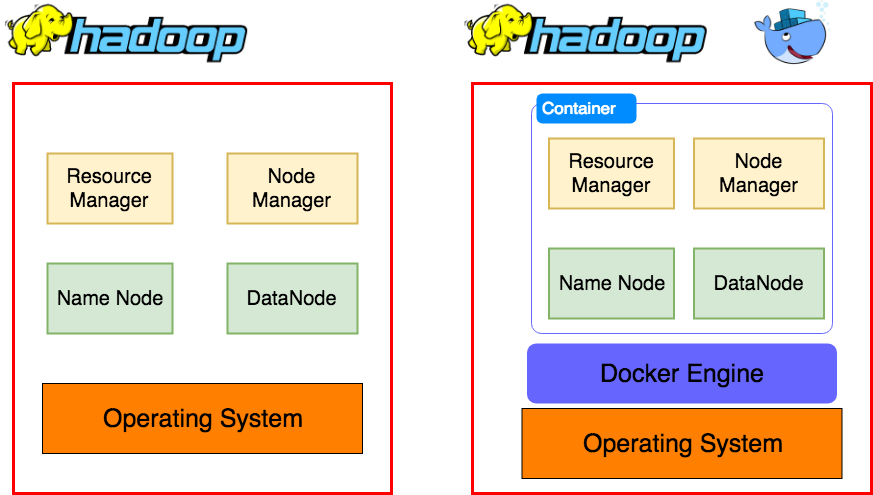
\includegraphics[width=\columnwidth]{images/hadoop-docker-pseudo.png}
	\caption{Architecture of Pseudo-Distributed 
	Hadoop}\label{f:hadoop-pseudo}
\end{figure}

\paragraph{Direct Installation}
Direct installation of Hadoop is done based on instructions on
Dominique Thiebaut's Wiki~\cite{hid-sp18-419-Thiebaut} and from The
Apache Software
Foundation~\cite{hid-sp18-419-Apache-single-node}. First a virtual
machine running Ubuntu 16.04 is setup on VirtualBox running on the
2017 Macbook Pro described in Section~\ref{ss:pcs}. It was decided to
increase the memory to 2GB and the virtual hard drive to 10GB based on
instructions provided in the Handbook~\cite{las18handbook}. Networking
is configured using a bridged adaptor connected to the host's wifi
port. OpenSSH, Curl, and the Java JDK 8 from OpenJDK are installed on
the VM. Per Thiebault's instructions, ipv6 is disabled. A group
called \verb|hadoop| is created with a user called \verb|hduser|. SSH
keys are created using \verb|ssh-keygen| and hduser's public key is
added to \verb|known_hosts| so that passwordless SSH to to localhost
is possible. Pyenv is then installed and python 3.6.2 is made the
global version of python for the VM. Hadoop 2.9.0 is downloaded from
Apache and installed in \verb|/usr/local/hadoop|. The following
environment variables are set in hduser's \verb|.bashrc| file:
\begin{verbatim}
export HADOOP_HOME=/usr/local/hadoop
export JAVA_HOME=/usr/lib/jvm/java-8-openjdk-amd64
\end{verbatim}

The following directories are added to hduser's path:
\begin{verbatim}
$HADOOP_HOME/bin
$HADOOP_HOME/sbin
\end{verbatim}

The rest of the configuration is done with modifications to xml files
and scripts in \verb|$HADOOP_HOME/etc/hadoop|: the java location needs
to be set in \verb|hadoop_env.sh|, the detault file system is set
in \verb|core-site.xml|, and the number of file system replications is
set in \verb|yarn-site.xml|. To make it easier to clean everything up
and rerun the algorithm, the directory used for temporary files is
also set in \verb|core-site.xml|.

The sentiment analysis algorithm was run in pseudo-distributed mode on
the VM with and without yarn as a resource manager. If yarn is used, a
few more configuratons need to be done in the xml files
in \verb|$HADOOP_HOME/etc/hadoop|: the mapreduce framework name needs
to be set to yarn in \verb|mapred-site.xml|,
and \verb|mapreduce_shuffle| needs to be set up
in \verb|yarn-site.xml|.

\paragraph{Dockerized Installation} We used a Dockerfile to build the 
image for the Pseudo-Distributed Hadoop container. The image is modified 
from the one on the sequenceiq github 
repository~\cite{hid-sp18-405-hadoop-sequenceiq}. The modification 
includes minor bug fixes, change of Java and Hadoop version, installation of 
Python and Pyenv, download of data and transfer of Python code for the use 
of Hadoop-Streaming. The container can be either started up with a shell 
interface for user to input commands operating the cluster or as an 
executable program which run the whole classification algorithm and transfer 
the results including running time back to the host machine. In later case, the 
docker container needs to be started by initiating a customized start-up 
script and overwrites the default scripts defined by the COMMAND or 
ENTRYPOINT settings in the Dockerfile. 


\subsection{Fully-Distributed using Docker Compose}

Fully-Distributed Hadoop cluster can be naturally deployed on multiple virtual 
and/or physical machines. However, the tool of Docker Compose makes it 
available to deploy the same mulit-node cluster on one single virtual machine. 
The architecture is illustrated in Figure~\ref{f:hadoop-compose}, where the 
red rectangle stands for some virtual or physical machine. This could be a 
personal laptop, VirtualBox running Ubuntu or FutureSystem Echo. However, 
since Echo is in Swarm mode, Docker Compose will only deploy the hadoop 
cluster on the head node, which conforms the restriction that only node 
interacting with clients is the head node. 

\begin{figure}[!ht]
	\centering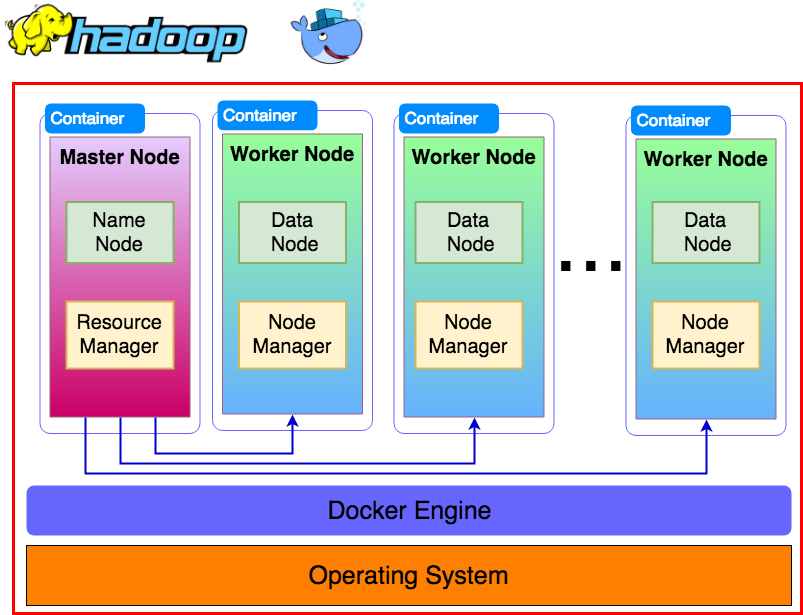
\includegraphics[width=\columnwidth]{images/hadoop-docker-compose.png}
	\caption{Architecture of Fully-Distributed 
		Hadoop Cluster Using Docker Compose}\label{f:hadoop-compose}
\end{figure}

In in Figure~\ref{f:hadoop-compose}, each Docker container acts as a node 
and the cluster contains one Master Node and 
multiple Worker Nodes. The ResourceManager and NameNode within the 
Master Node container could communicate with the all the NodeManagers 
and DataNodes respectively using TCP ports. 

The configuration process differs from the Pseudo-Distributed Hadoop 
container in two ways. First, there will be two different start-up scripts for 
Master Node container and Worker Node container respectively. The script 
for Master Node will only start ResourceManager and NameNode but not 
NodeManager or DataNode, and the script for Worker Node will do the other 
way around. Second, a YAML file needs to be configured with information of 
Master and Worker Node containers including image to use, ports to expose, 
network, container name, start-up command etc. One important feature 
Docker Compose provides is that one only need to configure one Worker 
Node containers in the YAML file instead of multiple ones. When starting up 
the service, a Docker Compose scale command can be used to scale up the 
number of Worker Nodes as desired. Furthermore, the scale command can 
also be used while the cluster is running. In that case, the number of Worker 
Nodes will be adjusted according to the scale command therefore the size of 
cluster can be controlled dynamically without the need of shutting down and 
restart the cluster. 

After the clusters are started up, user could log into any of the containers, 
check status, and run commands. We did also made the running of 
sentiment analysis algorithm automated in a similar way the 
Pseudo-Distributed cluster using Docker Containers.


\subsection{Fully-Distributed using Docker Swarm}

Although Docker Compose provides a way to simplify the deployment of a 
Fully-Distributed Hadoop cluster, the limitation is obvious. All the containers 
have to be on the same Docker Engine on an operating system, thus they are 
within the scope of the same virtual/physical machine. Therefore, the number 
of Worker Nodes and the computation and storage capability of the cluster is 
limited by the host machine (either virtual or physical). Docker Swarm as 
introduced in Section~\ref{s:techused}, provides a way to deploy the cluster 
across different machines. 

Instead of building a cluster of virtual machines with Docker Swarm enabled, 
for this project we used the FutureSystem Echo, where Docker Swarm has 
been fully implemented. The architecture of the Hadoop cluster is illustrated 
in Figure~\ref{f:hadoop-swarm}, where each red rectangle stands for a 
physical node other than the head node in the swarm cluster because Docker 
Swarm will not deploy any container on the head node. Although in this case, 
the Master Node will be on a different machine from some of the Worker 
Nodes, the communication is enabled within the network which is 
automatically built as the first step of the cluster deployment. 
Similarly as Docker Compose, the Swarm Mode also allows scaling up of the 
cluster without temporary shut down. 

\begin{figure}[!ht]
	\centering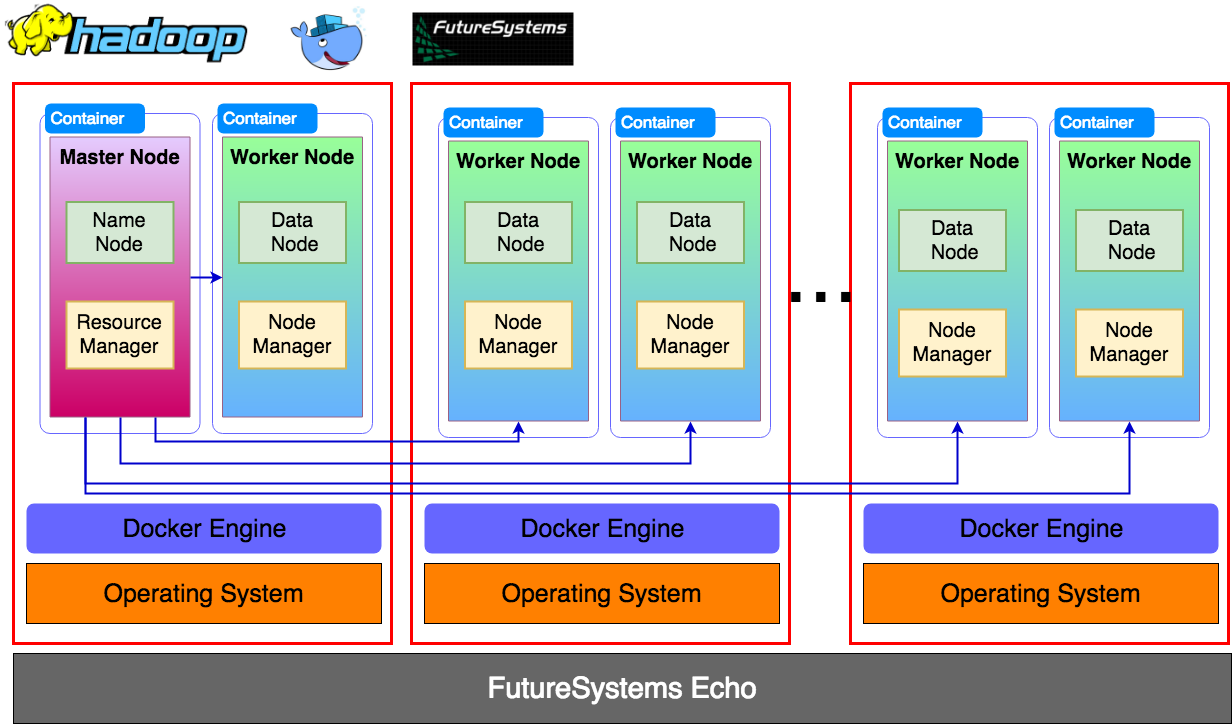
\includegraphics[width=\columnwidth]{images/hadoop-docker-swarm.png}
	\caption{Architecture of Fully-Distributed 
		Hadoop Cluster Using Docker Swarm}\label{f:hadoop-swarm}
\end{figure}

The YAML file for Docker Compose can be used to configure the cluster 
under the Swarm mode with some minor changes. Additional options such as 
deploy is available while some options are disabled such as container name. 
One key difference is that we have to include some start-up scripts and use 
those as Entrypoint or Command to make the algorithm of sentiment analysis 
run automatically when the cluster starts. Unlike in previous methods of 
deployment, where we still have the option of logging into the container and 
pass commands through bash, in swarm mode we cannot log into the 
containers because they are all deployed on worker nodes of the Swarm 
cluster. 

One caveat is how one could get the analysis results, which sits on some 
worker node in the Swarm cluster, back to the head node. One stardard way 
could be using the WebHDFS REST API with the curl command. However, in 
our implementation, we had a difficulty accessing different datanode, where 
the results are actually stored, through WebHDFS. This could be caused by 
some port issue and configuration in the initial HDFS setting. As a 
workaround, we put the results together with the log files in to the logs 
folder, which can be accessed through the YARN ResourceManager on 
certain port (8008 by default).


\TODO{Please check if the next paragraph is appropriate}
At the current state of this project, the Fully-Distributed Mode Hadoop 
clustersare achieved using Docker containers. As a future project, we 
planned to set up Raspberry Pi's clusters and each Pi acts like a node in 
Hadoop without virtualization. The Pi cluster set-up and initialization has 
been included in 
Section~\ref{s:appendix}.

\section{Benchmarking Process}\label{s:benchrproc}

The benchmarking has been done on several machines listed in 
Section~\ref{s:techused}, the 8GB ram Macbook Pro (mac for short), the 
16GB ram Asus laptop running centos (centos for short), the 16GB ram 
desktop with ubuntu Virtualbox (ubuntu for short), and FutureSystem Echo. 
For each of these machines, we used Docker to deploy Pseudo-Distributed 
Hadoop, and Fully-distributed Hadoop using Docker Compose for worker 
number starting at 1. For each setting, 10 iterations of the whole process of 
setting up cluster and running algorithm were performed. We then calculated 
the mean of running time together with standard deviations and the 
coefficient of variation (which is the ratio of standard deviation and mean). 
On echo, we also benchmarked the Fully-distributed Hadoop using Docker 
Swarm in a similar fashion. 

For some machines, there is a limit on the number of workers that can be 
established. For example, the mac can have at most two workers, otherwise 
the algorithm cannot be finished. The Java exceptions indicate that the 
machine ran out of memory. The two 16GB ram machines, centos and ubuntu 
could support 5 or 6 workers in a stable fashion. Stability here is defined as 
each iteration ending successfully and the deviation in running time is 
relatively small. Detailed results will be provided in Section~\ref{s:results}. 

\section{Results}\label{s:results}
This section elaborates the result of our benchmarking process, we will 
discuss deployment time and running time separately. 

\subsection{Deployment Time}

All the dockerized Hadoop cluster depends on Docker Engine and 
corresponding images. The Deployment can be divided into three steps. 

\begin{itemize}
	\item Install of Docker
	\item Build/Pull the image(s)
	\item Start the cluster
\end{itemize}

\paragraph{Install of Docker}
	The installation of Docker on Linux and MacOS operating systems 
	following the official guide on Docker website can be done in around 1 
	minute. 
	
\paragraph{Build/Pull the image(s)}	
	Based on different Internet connection speed we tried, one could build the 
	images for deployment from time range 8 to 12 minutes. Notice that the 
	images could also be pulled from DockerHub, which is the default 
	cloud-based registry service of Docker. In our test, Pulling in general is 
	faster than building images by around 1 minute. We have four images 
	throughout the whole project, namely pseudo, base, master and worker. 
	The majority of layers are the same with some differences such as Hadoop 
	configuration files, startup scripts, existence of data. Due to the share of 
	layers, building 3 images (base, master and worker) for the 
	Fully-Distributed cluster does not differ much from building only one. In 
	the future, we could unify all images into one, with different scripts or 
	options for the startup. It is noticed that on a single virtual machine, if the 
	iamges are pulled or built once, then later building process will utilize the 
	cached layers and speed up the process.
	
\paragraph{Startsthe cluster}
	Starting a Pseudo-Distributed Hadoop takes less than 10 seconds. The 
	start-up time for the Fully-Distributed cluster increases with the number of 
	workers initialized. For worker number smaller than 10, the start-up takes 
	less than 20 seconds. On FutureSystem  Echo, under either Compose or 
	Swarm mode, starting 40 workers took around 30 seconds and starting 
	100 workers took 40 seconds. 


From the breakdown of deployment steps, we could see that the build/pull 
image step dominates the total time of the whole process. The total time is 
not more than 13 minutes in total, building from scratch. In our project, we 
also deployed a Pseudo-Distributed Hadoop direclty (without Docker)  on a 
VirtualBox. The process of manually setting up hadoop with all dependencies 
and configuration files took much longer than the dockerized version. This 
illustrated the advantage of using Docker containers in cluster deployment. 


\begin{table}[hbt]
\centering
\caption{Benchmarking results}\label{t:results-table}
\begin{tabular}{llll}
Platform    & Docker & Deployment time & MapReduce Time \\
Pi 5 nodes  & Yes    & TBD             & TBD            \\
Pi 5 nodes  & No     & TBD             & TBD            \\
Echo        & Yes    & TBD             & TBD            \\
Echo        & No     & TBD             & TBD            \\
\end{tabular}
\end{table}



\section{Conclusion}\label{s:conclusion}

\TODO{Put here an conclusion. Conclusion and abstracts must not have any
citations in the section.}

\section{Appendix: Hadoop Cluster on Raspberry Pi}\label{s:appendix}
This section describes steps taken toward the goal of creating a
Hadoop cluster using 5 Raspberry Pi 3 Model B computers in a
repeatable, scalable way, so that the process could be replicated to
create a much larger cluster. Successes and challenges are described
and recommended next steps are outlined.

At the end of the process, each Pi has a unique hostname a new
password. A computer outside of the cluster can log into any of the
pis via ssh and the pis are configured to run mapreduce jobs using
Apache Hadoop. The process of achieving these goals manually has been
well documented in various blogs and message boards on the
internet~\cite{hid-sp18-419-headless}, but in order to make the
process scalable, the confuguration described is automated to a large
extent.

\subsection{Hardware Used}

The hardware used for the Raspberry Pi cluster consists of:

\begin{itemize}
\item Five Raspberry Pi 3 Model B computers 
\item One Waveshare 4in HDMI LCD touchscreen
\item One Netgear model GS308 8-Port Gigabit ethernet switch
\item One Anker PowerPort 6 USB power supply
\item One Powtech 125V AC 15A 1875w adaptor with switch
\item Five 1-foot ethernet cables
\item Five 32 GB microSDHC UHS-I cards
\item Six 6in USB 2.0 A-Male to Micro B cables
\item 24 20mm by 5mm Hex Hexagonal Threaded Spacer Supports
\end{itemize}

A pinout diagram of the Pi 3B is shown in Figure~\ref{f:pinout-diagram}.

\begin{figure*}[!ht]
  \centering\includegraphics[width=\columnwidth]{images/raspberry_pi_circuit_note_fig2.png} \caption{Pinout
  diagram of Raspberry Pi 3B~\cite{hid-sp18-419-pi-pinout}. Note: the
  Pi used for this project has a Broadcom BCM2837, not the Broadcom
  BMC2835 shown in this figure.}\label{f:pinout-diagram}
\end{figure*}

\subsection{Building a Pi Cluster}
First, aluminium and copper heat syncs need to be attached to each
Pi. The two aluminium heat syncs are attached to the Broadcom chip and
the SMSC ethernet controller located on the top of the Pi. The blades
of the heat syncs are parallel to the longer side of the Pi as shown
in Figure~\ref{f:heat-sync-top}.

\begin{figure*}[!ht]
  \centering\includegraphics[width=\columnwidth]{images/heat-sync-top.jpg} \caption{Top
  view of a Raspberry Pi 3B with heat syncs
  attached.}\label{f:heat-sync-top}
\end{figure*}

The flat copper heat sync is attached to the Elpida RAM on the bottom
of the Pi as shown in Figure~\ref{f:heat-sync-bottom}.

\begin{figure*}[!ht]
  \centering\includegraphics[width=\columnwidth]{images/heat-sync-bottom.jpg} \caption{Bottom
  view of a Raspberry Pi 3B with heat sync
  attached.}\label{f:heat-sync-bottom}
\end{figure*}

After attaching the heat syncs, threaded hexagonal spacer supports are
used to connect the Pis together. A fully-assembled 5-node Pi cluster
is shown in Figure~\ref{f:cluster-no-wires}.

\begin{figure*}[!ht]
  \centering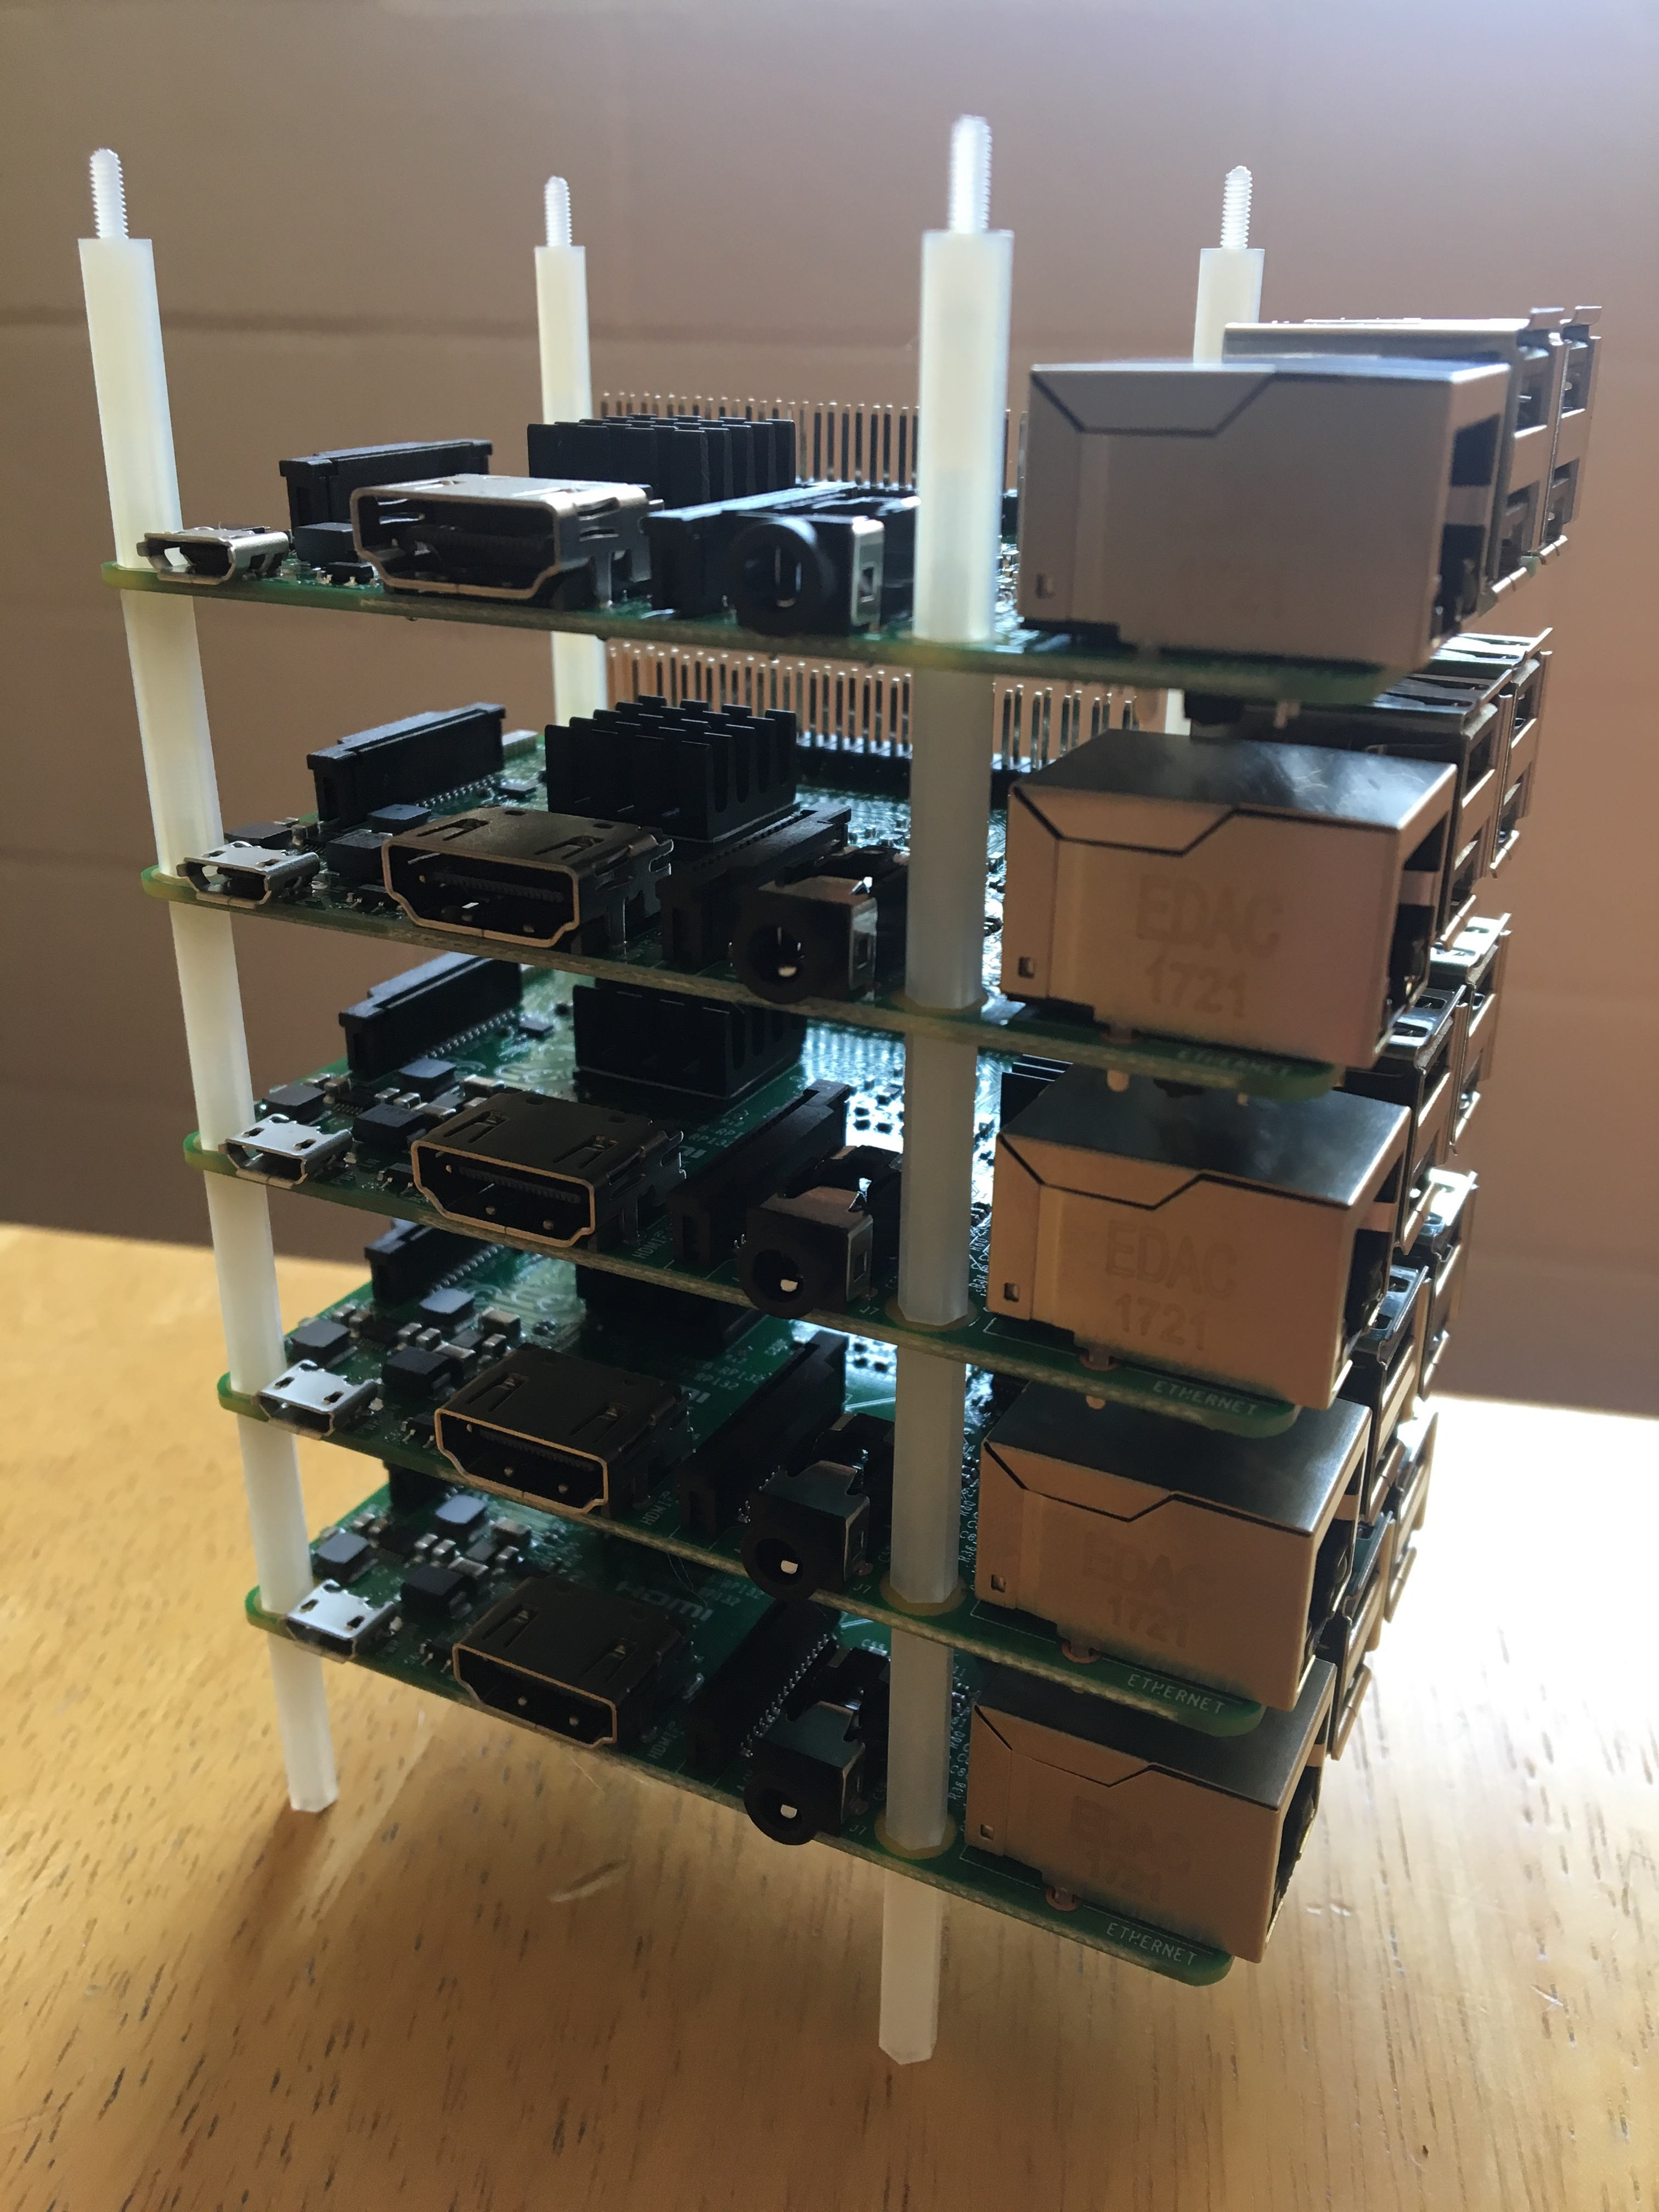
\includegraphics[width=\columnwidth]{images/pi-cluster-no-wires.jpg}
  \caption{5-node Pi cluster before wiring.}\label{f:cluster-no-wires}
\end{figure*}

Each node of the cluster is then attached to the switch using an
ethernet cables and to the power supply using a usb cables. The fully
wired cluster is shown in Figure~\ref{f:complete-cluster}.

\begin{figure*}[!ht]
  \centering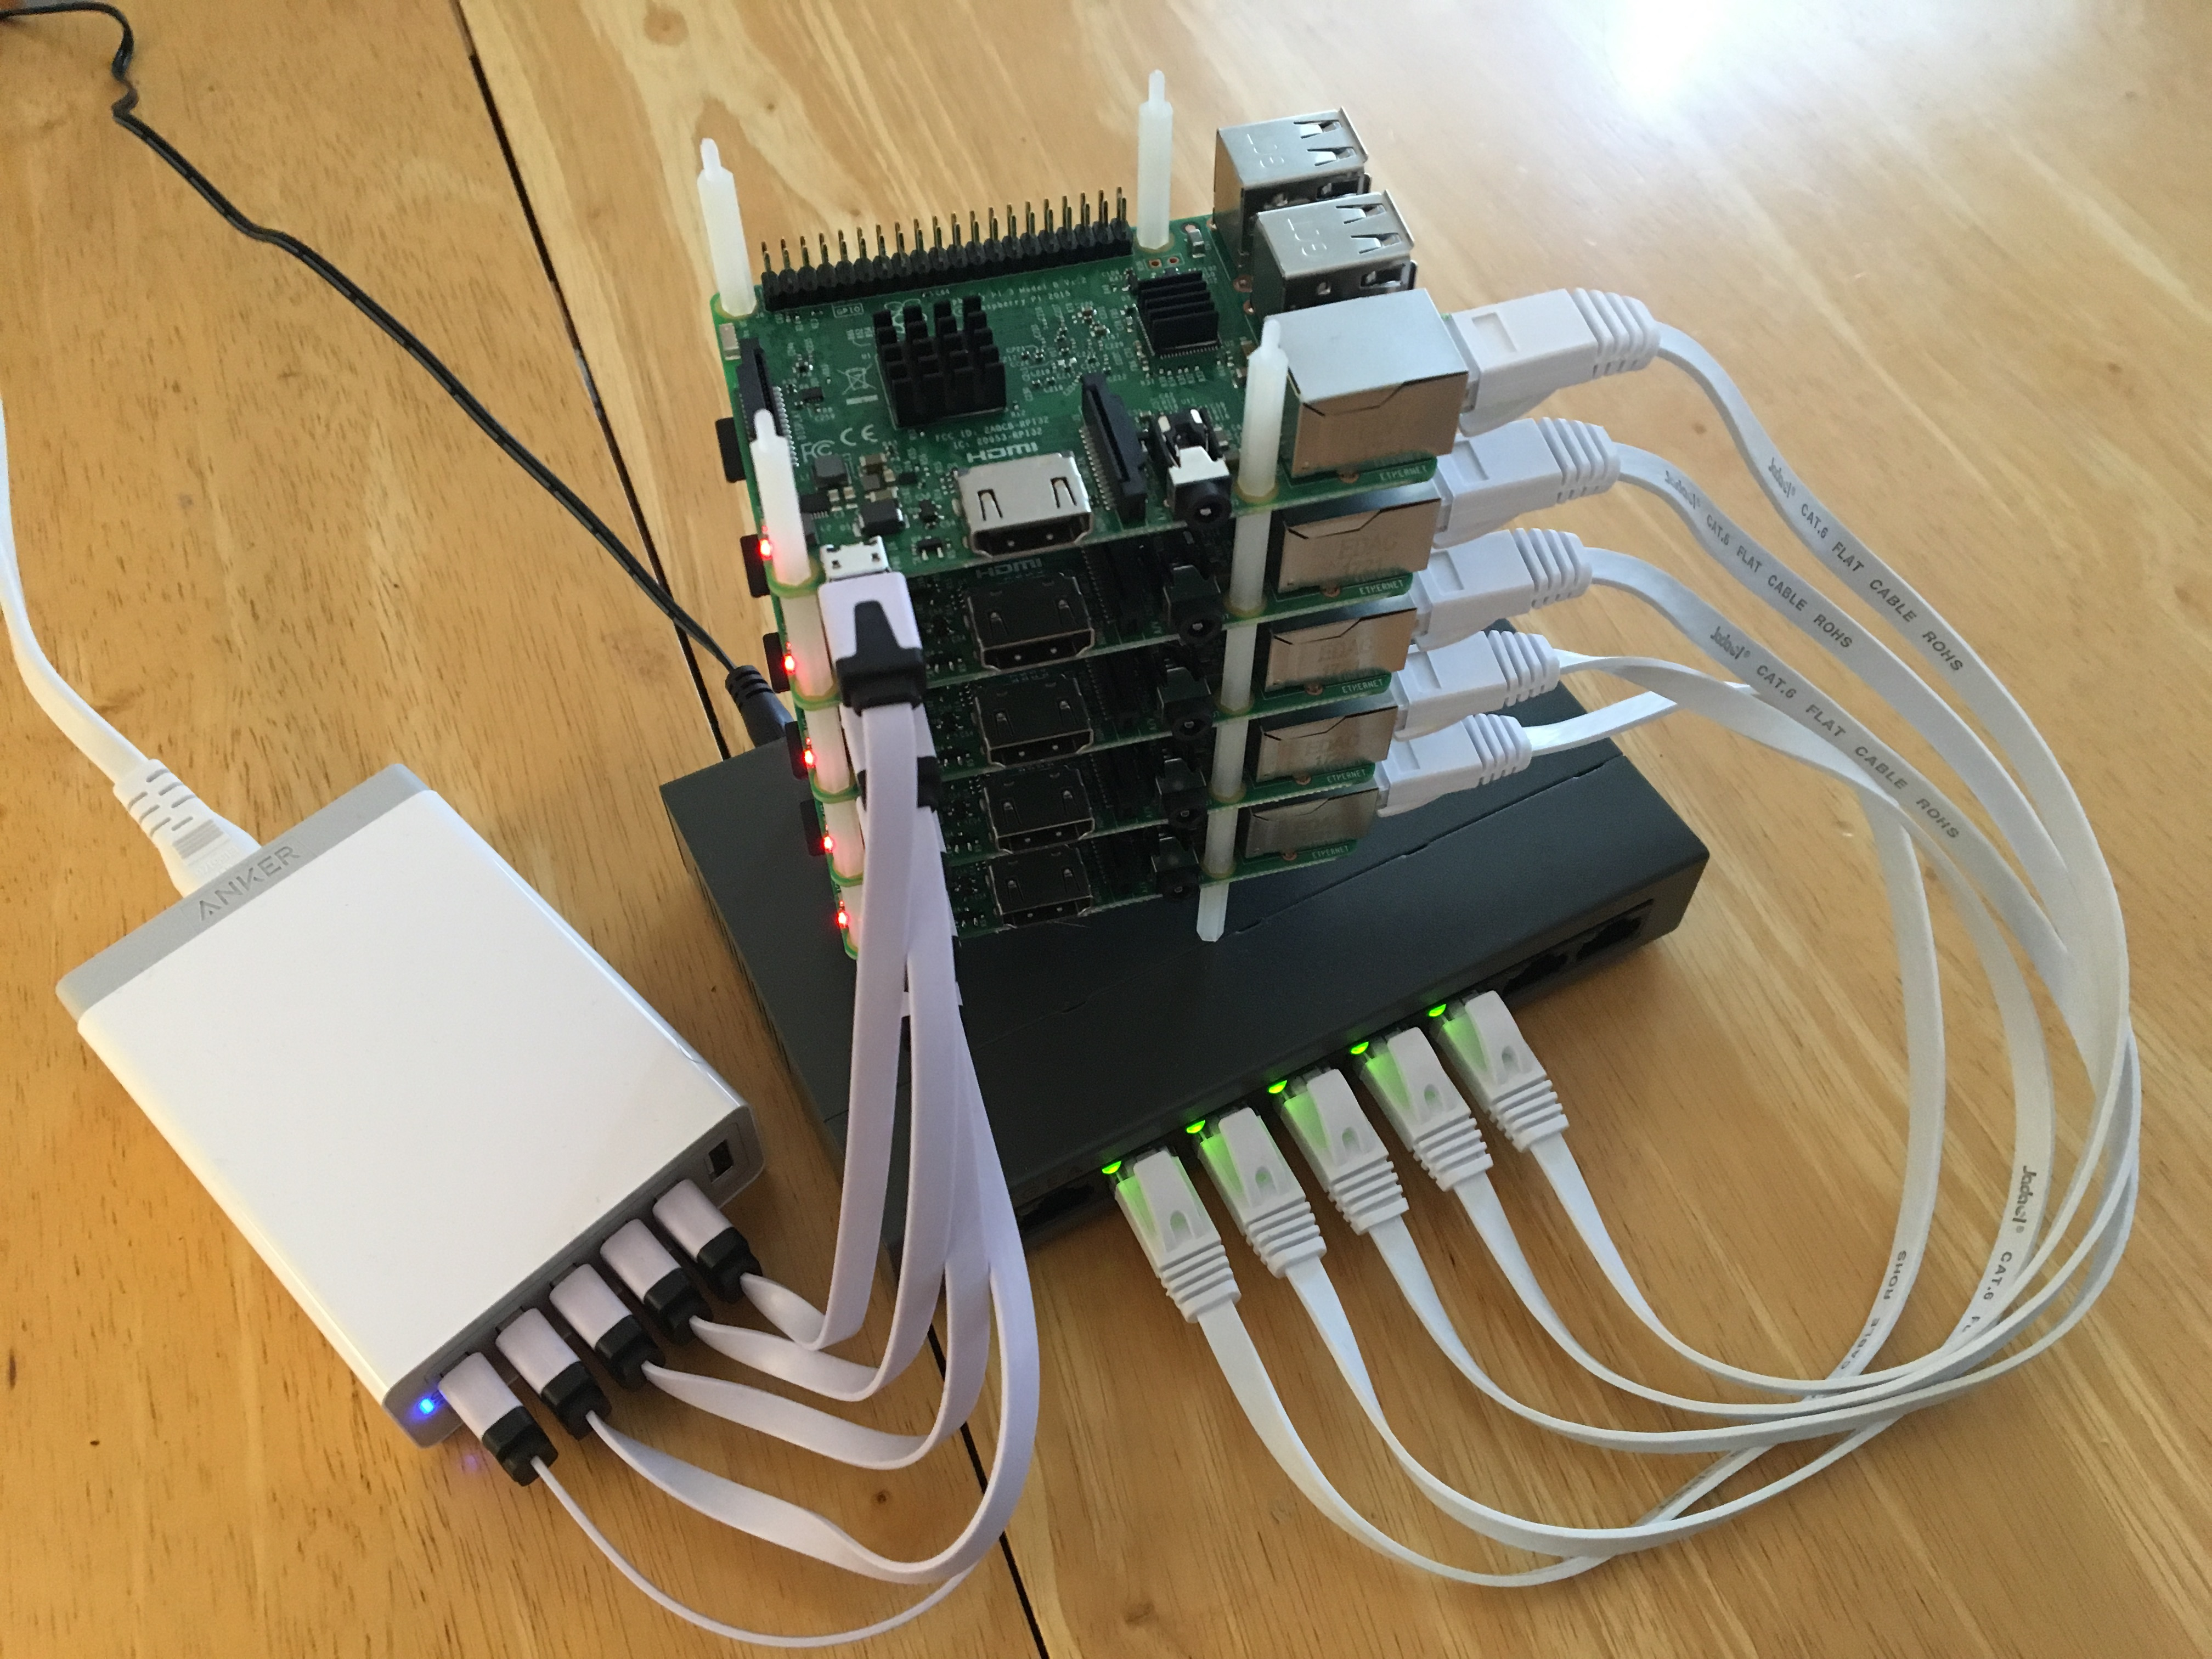
\includegraphics[width=\columnwidth]{images/complete-pi-cluster.jpg}
  \caption{Fully assembled 5-node Pi cluster.}\label{f:complete-cluster}
\end{figure*}

\subsection{Creating a Custom Image}
Each Pi uses a 32GB SD card as its hard drive. The operating system is
to be burned on each SD card. For this cluster, the most current
version of Raspbian Stretch Lite is chosen as the operating
system. When downloaded, this image has ssh disabled and is configured
with one user \verb|pi| with the password \verb|raspberry|. Every
machine is named \verb|raspberrypi|. In order to easily determine
which SD card is in which computer in the cluster, the names are
changed before burning the image to the SD card, and ssh is enabled on
each card so the rest of the configuraton can be done from a remote
computer without using a keyboard or monitor, commonly known as
headless setup.

Another approach that the authors would like to explore at a later
date would be to compile a custom image from the Raspbian source
code. The code is freely available to download, either directly from
raspbian.org~\cite{hid-sp18-419-raspbian-distro} or on
GitHub~\cite{hid-sp18-419-pi-gen}.

The computer used to create the custom images is the 2017 Macbook Pro
that is described in Subsection~\ref{ss:pcs}. The script that creates
the custom images downloads the latest image from Raspbian.org and
mounts the two partitions so that they can be modified. The process
used to mount the second partion only works on Linux, so a VM is
created on which the script is run. This VM needs to have a big enough
virtual disk for the base image times the number of custom images
created. The current unzipped Raspbian Stretch Lite image at the time
of this writing is 1.9GB. Instructions for setting up the VM provided
in the Handbook were used~\cite{las18handbook}.

If the images are going to be burned and verified on the VM,
additional space will be needed equal to the size of the SD cards
being burned because verificaton is done by copying the entire
capacity of the SD card and comparing it to the image that was
burned. The SD cards we are using are 32GB, so creating 5 images and
verifying the burn will require around 44GB on top of the space
required for Ubuntu. To be safe, the VM for creating the custom images
is configured with at least a 65GB virtual disk image hard drive.  It
runs Ubuntu 16.04 on VirtualBox and is configured with 1 CPU, 2GB of
memory, and USB 3.0 enabled. Networking is via a bridged network
connected to the hosts WiFi.

The images are created using two scripts: \verb|download_image.sh| - a
simple shell script to download the latest Raspbian Stretch Lite
image, and \verb|modify_sdcard.py| - a python script that will create
the custom images. The python script runs on python version 2.7.12,
which is the version that comes installed on Ubuntu 16.04. It requires
one additional package, \verb|pycryptodome|, which is needed to
generate ssh keys. The script needs to be run as root to have
permission to mount and modify the files in the Raspbian image.

The python script creates the number of custom images specified with a
flag. The names of the images are a basename followed by a three-digit
number that increments sequentially from the specified starting number
through that number plus the number of images created. The basename,
starting number, and number of images can be specified with flags. The
basename defaults to \verb|snowcluster| and the starting number
defaults to 0, so if three images were specified, the result would be
three files: \verb|snowcluster000.img|, \verb|snowcluster001.img|,
and \verb|snowcluster002.img|.

When the script is run, the base image is copied the number of times
specified by the user and the following modifications are made: * If
the \verb|--ssh| flag is set, or by default, the script will mount the
first partition of the image and add a blank file
named \verb|ssh|. This enables ssh on the Pi on first boot. It also
generates public and private RSA keys, creates a
folder \verb|//home/pi/.ssh/| and stores those keys in files
called \verb|id_rsa| for the private key and \verb|id_rsa.pub| for the
public key. It then appends the public key to the
file \verb|/home/pi/.ssh/authorized_keys|. If that file does not yet
exist, it is created. This allows passwordless ssh login between any
of the Pis in the cluster.  * If the user specifies a public key with
the \verb|--sshkey| flag, the contents of that file is also appended
to the file \verb|/home/pi/.ssh/authorized_keys|. This allows
passwordless ssh into the any of the Pis in the cluster from a setup
machine.

After the images are created, they can either be copied to a shared
folder and burned to the SD cards on the Mac using Etcher, or on the
VM using \verb|dd|. Instructions for doing this provided by The
Raspberry Pi Foundation were tested on both
platforms~\cite{hid-sp18-419-raspbian-burn}.

A known issue with the python script is that because it needs to be
run as root to mount and unmount the images and modify the
contents, \verb|~/.ssh| and its contents: \verb|id_rsa|,
\verb|id_rsa.pub|, and \verb|authorized_keys| are owned by root.
This leads to a permissions error when connecting via ssh from one pi
to another. Solutions for this issue need to be investigated.

In addition to fixing this permissions issue, other desired future
enhancements include:

\begin{itemize}
        \item Adding an option to specify paramaters in a yaml file as
        specifying them on the command line is cumbesome.
        \item Adding an option to create keys and adding them
        to \verb|known_hosts| on all the images to bypass the
        verification on first ssh connection.
        \item Setting a fixed
        IP address on the head node if DHCP is to be used, or for all
        the Pis.
        \item Incorporating the functionality
        in \verb|download_image.sh| into script, with option to
        download a different base OS (e.g. from Dexter Labs).
        \item Adding an option to burn the images from the script.
        \item Adding a script to do post-boot configuraton.
\end{itemize}

\subsection{Post-boot configuraton}
Post-boot configuration was explored but not implemented. The goal for
future development would be to write a script that would perform the
remainder of the configuration, copy it to each of the Pis, and run on
first login. This script will permanently enable ssh; change the
password of all of the Pis; create or update a database containing IP
addresses, Mac addresses, and hostnames; optionally configure the head
node of the cluster as a DHCP server; and install and configure Hadoop
on the Pis.

Permanently enabling ssh is necessary as the \verb|ssh| file added in
to the first partition is deleted after first login. It is done with
the following commands:
\begin{verbatim} 
sudo apt-get update
sudo apt-get install openssh-server
sudo systemctl enable ssh
sudo systemctl start ssh
\end{verbatim}

Changing the password from the default password \verb|raspberry| to
something more secure can be done with this
line~\cite{hid-sp18-419-so-password}:
\begin{verbatim} 
echo -e ``raspberry\\nsnowcluster\\nsnowcluster'' | passwd
\end{verbatim}

The database of Mac addresses, IP addresses, and hostnames can be done
in two steps: populate the hostnames and IP addresses during the
creation of the VM images, and add the Mac addresses after booting up
the Pis. Then the setup script can run \verb|ifconfig -a| and parse
the output to get the Mac addresses for both wireless and wired
connections. The output of ifconfig -a is shown in below.
\begin{verbatim} 
eth0: flags=4163<UP,BROADCAST,RUNNING,MULTICAST>  mtu 1500
        inet 192.168.2.7  netmask 255.255.255.0  broadcast 192.168.2.255
        inet6 fe80::ed2:8b8e:f74a:d698  prefixlen 64  scopeid 0x20<link>
        ether b8:27:eb:00:c3:55  txqueuelen 1000  (Ethernet)
        RX packets 264  bytes 43987 (42.9 KiB)
        RX errors 0  dropped 0  overruns 0  frame 0
        TX packets 87  bytes 14502 (14.1 KiB)
        TX errors 0  dropped 0 overruns 0  carrier 0  collisions 0

lo: flags=73<UP,LOOPBACK,RUNNING>  mtu 65536
        inet 127.0.0.1  netmask 255.0.0.0
        inet6 ::1  prefixlen 128  scopeid 0x10<host>
        loop  txqueuelen 1000  (Local Loopback)
        RX packets 0  bytes 0 (0.0 B)
        RX errors 0  dropped 0  overruns 0  frame 0
        TX packets 0  bytes 0 (0.0 B)
        TX errors 0  dropped 0 overruns 0  carrier 0  collisions 0

wlan0: flags=4099<UP,BROADCAST,MULTICAST>  mtu 1500
        ether b8:27:eb:55:96:00  txqueuelen 1000  (Ethernet)
        RX packets 0  bytes 0 (0.0 B)
        RX errors 0  dropped 0  overruns 0  frame 0
        TX packets 0  bytes 0 (0.0 B)
        TX errors 0  dropped 0 overruns 0  carrier 0  collisions 0
\end{verbatim}

The Mac addresses for the Pis begin with \verb|b8:27:eb:|. The wired
Mac address is shown above in the third line under \verb|eth0|
as \verb|b8:27:eb:00:c3:55| and the wireless Mac addres in the third
line below \verb|wlan0| as \verb|b8:27:eb:55:96:00|.

Setting up head node of the cluster as a DHCP server requires further
investigation and testing. The process was followed and documented,
but a new version of the DHCP server \verb|isc-dhcp-server| is
incompatible with the process followed~\cite{hid-sp18-419-pi-DHCP}.

\section{Work Breakdown}
Min Chen converted the sentiment analysis algorithm, did the Docker
configurations and benchmarking and was the main author of these
sections of the paper. Bertolt Sobolik did the Pi configuration and
pseudo-distributed configurations on the virtual machines and was the
main author of these sections of the paper. Min Chen and Bertolt
Sobolik review and tested each other's work.

\begin{acks}

  The authors would like to thank Dr.~Gregor~von~Laszewski for his
  support and suggestions to write this paper, and Bo Feng for his guidance 
  and help with Hadoop deployment in Docker Swarm mode.

\end{acks}

\bibliographystyle{ACM-Reference-Format}
\bibliography{report}
